\chapter{Approach}
\label{ch:approach}
In the following section, we introduce our proposed security approach for substation automation systems.
With the aim of securing the time-critical communication between resource-constrained devices in a time-variable environment, we propose a \textbf{C}ertificateless \textbf{A}ttribute-Based \textbf{S}erver-Aided \textbf{C}ryptosystem for \textbf{S}ubstation \textbf{A}utomation \textbf{S}ystems (CASC-SAS).
The CASC-SAS cryptography and cybersecurity approach is able to prevent and mitigate cyberattacks by providing security schemes and mechanisms, and enforcing mandatory communication policies.

The goal of the approach is the enhancement of SAS security by providing secure authentication, authorization, and attribute-based access control for time-critical SAS communication.
The CASC-SAS approach comprises two core concepts.
The first core concept of the approach is the Certificateless Attribute-Based Server-Aided Authentication (CASA), which is further discussed in \autoref{sec:approach:casa}.
The second core concept of the approach is the Server-Aided Attribute-Based Authorization and Access Control (SABAAC), which is further discussed in \autoref{sec:approach:sabaac}.
Moreover, the approach is based on a dual-path four-layered architecture.
The two paths are referred to as data path and control path.
The four layers of the architecture are referred to as domain, cybersecurity, cryptography, and message exchange.
The architectural layers are illustrated in \autoref{fig:layers_request_example}.
\begin{figure}
    \centering
    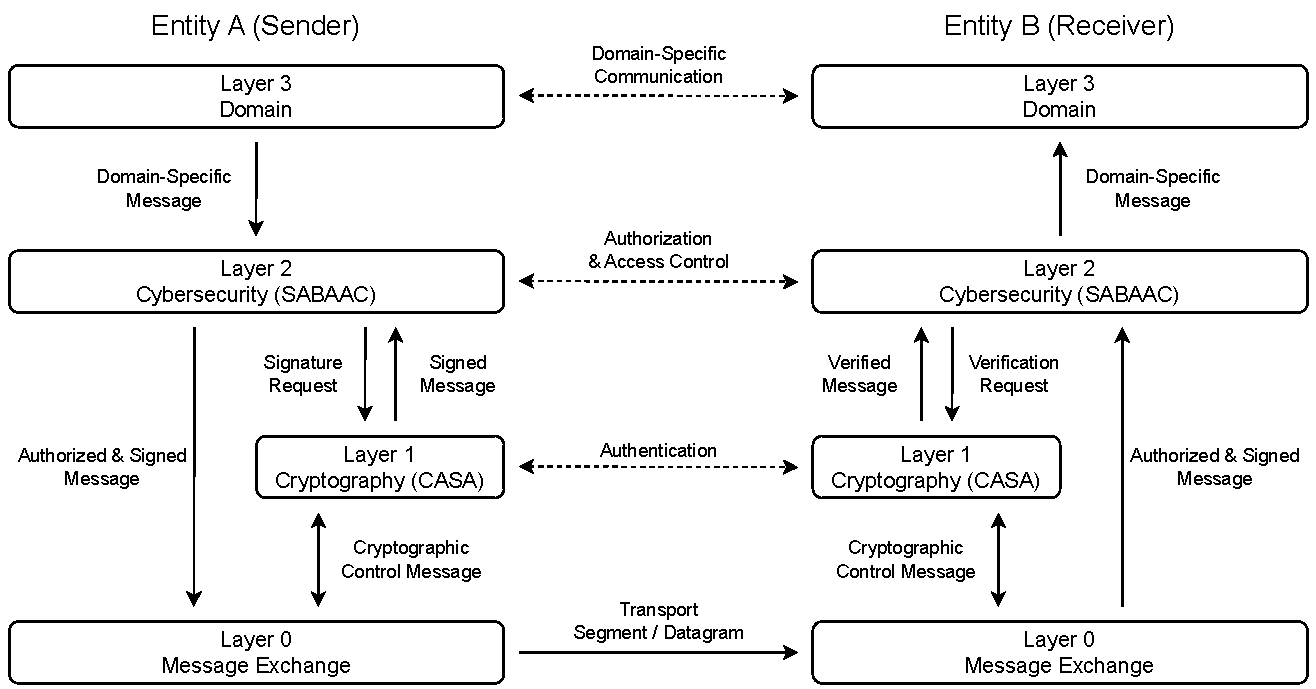
\includegraphics[width=0.8\linewidth]{figures/layers_request_example.drawio.pdf}
    \caption{Exemplary message exchange in four-layered CASC-SAS architecture.}
    \label{fig:layers_request_example}
\end{figure}

\section{Requirements}
In the following, we introduce the requirements of the presented approach.
Based on the identified requirements, functional and non-functional characteristics of the proposed approach are derived and evaluated.
Each requirement is associated with a requirement category.
The requirement categories consist of security, safety, availability, performance, and compatibility.

With regard to information security the approach has to satisfy seven requirements, namely device integrity, message integrity, authenticity, access control, non-repudiation, Principle of Least Privilege (PoLP), and Separation of Duties (SoD).
With regard to safety the approach has to satisfy operational safety and fail-safe requirements.
With regard to availability the approach has to satisfy operational continuity and fail-operational requirements.
With regard to performance the approach has to take three constraints into account, namely communication latency, computational complexity, and energy as well as power.
With regard to compatibility the approach has to satisfy interoperability and interchangeability requirements.

\section{Certificateless Attribute-Based Server-Aided Authentication (CASA)}
\label{sec:approach:casa}
In the following section, we present the \textbf{C}ertificateless \textbf{A}ttribute-Based \textbf{S}erver-Aided \textbf{A}uthentication (CASA) concept.
CASA is a CL-PKC approach.
The goal of CASA is to provide cryptographic algorithms and schemes for key generation, key distribution, key revocation, signing, and verification.
Moreover, the goal of CASA is to enable and support more abstract cybersecurity mechanisms like authorization and access control of the CASC-SAS approach.
Therefore, CASA represents the foundation of the employed CASC-SAS cybersecurity mechanisms.

Since CASA is a CL-PKC approach, neither certificates nor key escrow is required~\cite{AlRiyami2003}.
Moreover, the CASA approach proposes a key generation that is not only based on subject identities but rather enables public keys and private keys based on arbitrary attributes of subjects or even groups of subjects.
The key generation of the CASA approach is inspired by the alternative CL-PKC key generation technique proposed by \citeauthor{AlRiyami2003} \cite{AlRiyami2003}.
The defining characteristics of the alternative key generation is the derivation of partial private keys from public keys and identities.
As a consequence, an entity has to generate its public key before it can request a partial private key from the KGC.
This alternative key generation enables sending of partial private keys over unsecure channels and reduces the required trust in the KGC.
Furthermore, this technique allows only one public key to be created for a specific private key.

\subsection{Server-Aided Cryptography}
As PKC mechanisms may consist of computationally complex algorithms and operations such as bilinear pairing, we propose a server-aided PKC approach.
Therefor, we propose an extension of the CL-PKC concept and schemes to make time-critical steps server-aided.
To make CASA server-aided, an Untrusted Cryptography Server (UCS) supports devices by handling computationally expensive algorithms instead of executing them locally on resource-constrained devices.
To minimize the required trust, the UCS may only handle certain computations, i.e., partially sign or verify a request of a device.
This server-aided approach enables resource-constrained devices to apply secure algorithms and schemes of CASA in a time-critical OT environment.
In the following, we employ the concept of server-aided PKC for the verification process.

A server-aided verification process has to satisfy the property of being computation-saving \cite{Wu2008}.
A server-aided verification process $V_{Aided}$ is computation-saving if the computational costs for the verifier are strictly less than the costs of non-server-aided verification $V_{Conventional}$.
In other words, $V_{Aided}$ is computation-saving if the equation $Cost(V_{Aided}) < Cost(V_{Conventional})$ holds.

\subsection{Online \& Offline Cryptography}
Since CASA is tailored for time-critical communication, the approach aims to reduce the required time for cryptographic algorithms.
In addition to server-aided cryptography, this time reduction is achieved by precomputation.
For this purpose, each step of an algorithm is classified as either online or offline.
Online steps depend on the sender's public key, the digital signature, or the message.
Consequently, online steps cannot be precomputed.
Nevertheless, specific online steps can be accelerated via server-aided cryptography.
Offline steps depend on information that is available before any message exchange occurs.
Therefore, offline steps can be precomputed to reduce the required time for cryptographic algorithms.

\subsection{Signature Scheme $\mathcal{S}_{CASA}$}
The CASA signature scheme $\mathcal{S}_{CASA} = (I, G_{VAL}, G_{PK}, G_{PPK}, G_{SK}, S, V_{ENT}, V_{SAV}, V_{FIN})$ is a nine-tuple of algorithms.
The algorithms comprise an initialization algorithm $I$, a secret value generation algorithm $G_{VAL}$, a public key generation algorithm $G_{PK}$, a partial private key generation algorithm $G_{PPK}$, a private key generation algorithm $G_{SK}$, a signing algorithm $S$, a partial entity verification algorithm $V_{ENT}$, a partial server verification algorithm $V_{SAV}$, and a final entity verification algorithm $V_{FIN}$.

\subsection{Security Model}
The proposed signature scheme $\mathcal{S}_{CASA}$ is a secure signature scheme if it is existentially unforgeable under an adaptive chosen-message attack (EUF-CMA)~\cite{Boneh2023, Goldwasser1988}.
To create an existential forgery, i.e., output a valid pair of message and signature for a new message, an adversary carrying out a CMA can request valid signatures from an entity for any message of his choice.
While non-adaptive CMA restricts the adversary to a fixed set of messages chosen prior to the attack, adaptive CMA allows the adversary to request signatures of messages depending on previously obtained signatures.

\section{Server-Aided Attribute-Based Authorization \& Access Control (SABAAC)}
\label{sec:approach:sabaac}
The second core concept of CASC-SAS is the \textbf{S}erver-Aided \textbf{A}ttribute-\textbf{B}ased \textbf{A}uthorization and \textbf{A}ccess \textbf{C}ontrol (SABAAC).
The SABAAC approach enables the employment of attribute-based authorization and access control for time-critical SAS communication.
Therefore, the approach prevents unauthorized access and extraction of information.
The approach enables CASC-SAS to satisfy the access control, PoLP, and SoD security requirements.
Moreover, the expressive and flexible but yet computationally expensive ABAC policies are handled in a server-aided manner to satisfy the strict time constraints of the SAS domain.

Our authorization and access control approach represents a cybersecurity concept that is located on the cybersecurity layer of the CASC-SAS architecture.
Since the approach is located on the cybersecurity layer, it relies on secure authentication services provided by CASA.
As a consequence, the approach assumes that efficient and secure signing and verification algorithms are available.
In other words, CASA provides secure cryptographic algorithms and schemes that enable SABAAC to realize secure authorization and access control.

\subsection{Authorization \& Access Control Architecture}
The proposed authorization and access control approach is based on a function-oriented component-based architecture.
The architecture consists of four functional units.
These functional units have been adapted from the access control mechanism functional points presented by \citeauthor{Hu2014} \cite{Hu2014}.
Each functional unit is represented by a component that offers function-oriented services.
The components of the architecture are TTPs since the semantic validity of their provided services is not verifiable by the service consumers.
An overview of the SABAAC architecture, components, and protocols as well as the integration of CASA components and services into the SABAAC approach are shown in \autoref{fig:sabaac_protocols_overview}.

Furthermore, SABAAC is divided into two central tasks or protocols.
The first task is referred to as delegated attribute-based authorization.
The delegated attribute-based authorization is responsible for the access control policy creation, management, storage, and distribution.
This process partially takes place prior to occurring access requests and corresponding access decisions.
The second central task is referred to as delegated ABAC.
The delegated ABAC is responsible for the policy decision exchange and policy enforcement.
This process takes place when an entity initiates the communication with another entity.
\begin{figure}
	\centering
    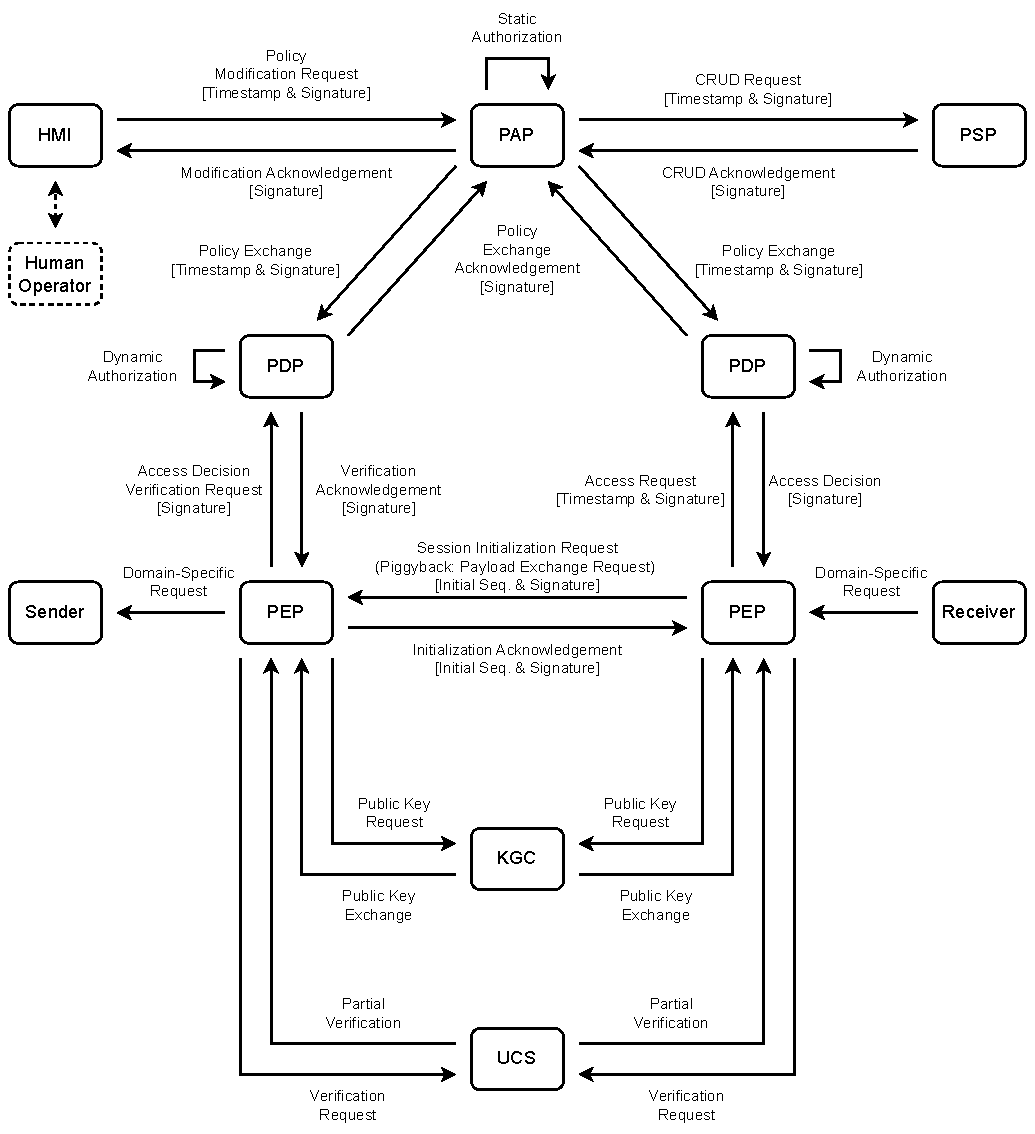
\includegraphics[width=0.8\linewidth]{figures/SABAAC_protocols_overview.drawio.pdf}
	\caption{Function-oriented component-based architecture of the SABAAC approach.}
	\label{fig:sabaac_protocols_overview}
\end{figure}

\subsection{Access Control Policy}
\label{sec:approach:sabaac:policy}
The SABAAC approach relies on the concept of attribute-based policies and access control due to the following benefits:
ABAC enables multifactor policy expression, while RBAC and IBAC limit the policy expressiveness by only relying on either roles or identities.
Consequently, the multifactor policy expression enables fine-grained and flexible access control.
Moreover, the use of ABAC can avoid explicit authorizations prior to a request \cite{Hu2014}.
This dynamic evaluation allows the use of attributes from a time-variable environment.
A so-called real-time attribute represents an attribute whose value is time-dependent \cite{Burmester2013}.
Given an attribute evaluation function $E_{ATT}$ and a point of time $t$, the value $\lambda_a$ of a real-time attribute $a$ is defined by $E_{ATT}(a, t) = \lambda_a$.
To handle policies based on their degree of time-variability, the SABAAC approach classifies policies as follows:
\begin{description}
    \item[Dynamic Policy] A dynamic policy $\rho$ is an ABAC policy whose evaluation relies on at least one time-variable subject, object, environment, or action attribute.
    A policy $\rho$ is dynamic iff $\exists a \in \rho: \exists t_i \neq t_j: E(a,t_i) \neq E(a,t_j)$.
    Due to the time-variable evaluation of dynamic policies, access decisions must have a limited time of validity that corresponds to the change rate of the underlying attribute values.
    As a result, caching of access decisions that are based on dynamic policies should be avoided.
    A dynamic policy is also referred to as real-time policy.
    \item[Static Policy] A static policy $\rho$ is an ABAC policy whose evaluation does not rely on time-variable subject, object, environment, or action attributes.
    A policy $\rho$ is static iff $\forall a \in \rho: \forall t_i,t_j: E(a,t_i) = E(a,t_j)$.
    Since static policies do not rely on time-variable attributes, access decisions can be cached.
    Moreover, due to the non-frequent attribute retrieval and evaluation as well as access decision caching, static policies are a viable solution for low latency message exchange.
    A static policy is also referred to as non-real-time policy.
\end{description}

\section{Realization}
\label{sec:approach:realization}
In the following section, we discuss the proposed realization of the CASC-SAS approach and its two core concepts CASA and SABAAC.
The approach and its two concepts introduce components that are defined and discussed in \autoref{sec:approach:casa} and \autoref{sec:approach:sabaac}.
These components have to be integrated into the SAS architecture to employ the CASC-SAS approach.
This integration of CASC-SAS components into the SAS architecture is visualized in \autoref{fig:casc_architecture}.
The components depicted in blue represent elements of the SAS architecture, whereas the components depicted in red are introduced by the CASC-SAS approach.
The components with a color gradient represent elements of the SAS architecture that have been adapted to support CASC-SAS concepts.
The PEP, PDP, UCS, and KGC components have to be present locally in every adapted SAS.
This is necessary due to the strict time constraints of SAS-internal low latency message exchange.
The PAP and PSP instances may be centrally deployed, since static authorization is part of the non-time-critical control path communication.
Any non-intermediate SAS component that participates in a communication relationship must either support the CASC-SAS protocols or use the services provided by a PEP to secure occurring message exchanges.
\begin{figure}
    \centering
    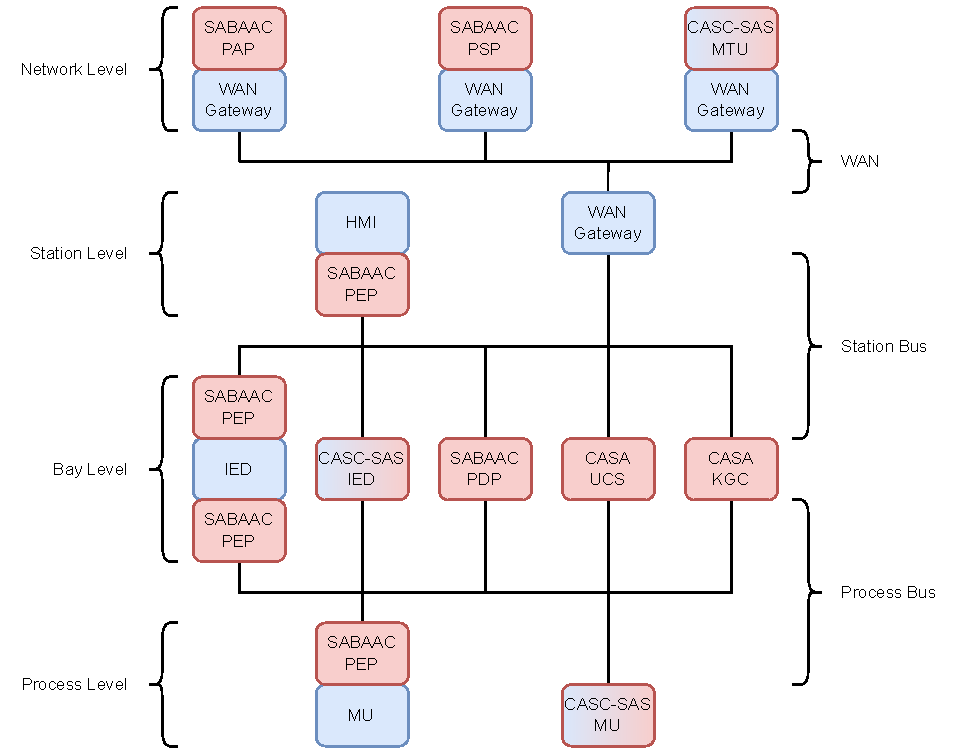
\includegraphics[width=0.8\linewidth]{figures/casc_architecture_color.drawio.pdf}
    \caption{Adaptation of the layered SAS architecture to the CASC-SAS approach.
    }
    \label{fig:casc_architecture}
\end{figure}

To examine the feasibility and perform the above-mentioned integration, we propose a hardware and software realization of our approach.
The aim of the realization is to provide implementations of CASA and SABAAC with a full range of functions.
The software is going to be implemented component-wise using high-level programming languages.
Depending on the complexity and time constraints of a specific component, different programming languages might be used for the implementation.
Due to internal dependencies, the software implementation is split into two parts.
The first part is dedicated to the CASA approach, as it represents the foundation of all employed protocols.
The second part is dedicated to the SABAAC components and protocols.

The employed components of CASA and SABAAC provide different services.
Furthermore, the components have to be deployed differently to correspond to the proposed protocols.
While PAP and PSP may be deployed centrally, components such as PEP, PDP, UCS, and KGC are distributed to individual SAS instances.
This leads to differing hardware requirements for the implemented components.
Moreover, except for PEP instances, the components provide their services by using a client-server pattern.
The PEP instances partially use a client-server pattern and partially provide their services in the form of a Bump-In-The-Wire (BITW) solution.
The services provided by PEP instances via BITW pattern are automatically applied to captured packets.
Therefore, these services are invisible to the corresponding service consumers.
This BITW pattern is inspired by the security filter approach presented by \citeauthor{Ishchenko2018} \cite{Ishchenko2018}.
Taking the differing provision patterns and deployment structures into account, we propose the usage of performance-oriented server hardware for the PAP, PSP, PDP, UCS, and KGC to avoid bottlenecks and mitigate the risk of accidental or malicious DoS.
Moreover, we propose the usage of inexpensive off-the-shelf hardware for the highly distributed PEP instances.

\section{Evaluation}
\label{sec:approach:evaluation}
In this section, the evaluation of the CASC-SAS approach is discussed.
The goal of the evaluation is to derive quantitative and qualitative metrics of the approach for different areas of interest.
These metrics are used to verify the applicability and to identify limitations of the proposed approach.
We propose three areas of interest for the evaluation of the CASC-SAS approach:
\begin{description}
    \item[Security Evaluation] Does CASC-SAS provide security against typical SAS adversaries and attacks?
    Which security, safety, and availability requirements are satisfied?
    Which system and adversary characteristics were assumed?
    Did the attack surface change?
    \item[Performance Evaluation] Is CASC-SAS capable of securing time-constrained communication of an SAS?
    Which performance requirements are satisfied?
    Which communication characteristics were assumed?
    Which types of messages are supported?
    Is the approach resistant against network exceptions including congestion, delay, jitter, duplicated packets, lost packets, and out-of-order packet delivery?
    \item[Compatibility Evaluation] Is CASC-SAS a feasible solution for the construction or retrofitting of an SAS?
    Which compatibility requirements are satisfied?
    Which device characteristics were assumed?
    How high are the additional costs for SAS construction and retrofitting?
\end{description}

\begin{figure}
    \centering
    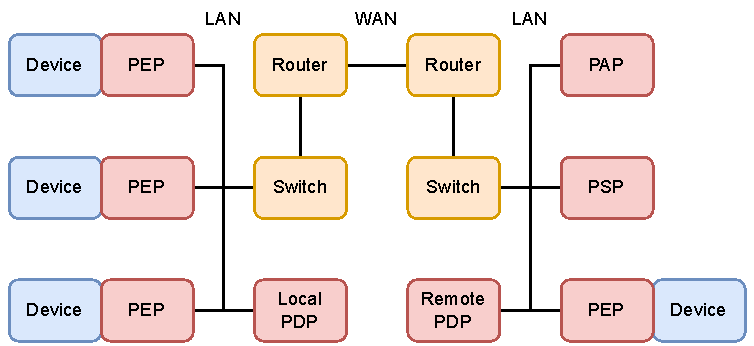
\includegraphics[width=0.7\linewidth]{figures/network_testbed_color.drawio.pdf}
    \caption{Architecture of the network test bed.}
    \label{fig:evaluation_test_bed}
\end{figure}
The evaluation is performed theoretically as well as experimentally.
For the theoretical parts of the evaluation, formal and informal methods are used to proof certain characteristics of the proposed approach.
The experimentally performed part of the evaluation is based on the realization presented in \autoref{sec:approach:realization}.
Based on the realization, a network simulation and network test bed, visualized in \autoref{fig:evaluation_test_bed}, are constructed.
The simulation strategy has the advantage of repeatability and reproducibility due to deterministic behavior, whereas the behavior of the test bed is non-deterministic.
The test bed results are practice-oriented and transferable to the physical SAS domain, whereas the behavior of a real SAS cannot be compared to the deterministic behavior of the network simulation.

